%!TEX TS-program = Arara
% arara: lualatex
% arara: biber
% arara: lualatex
% arara: lualatex

\documentclass[12pt,ngerman]{scrbook}

\usepackage[utf8]{inputenc}
\usepackage[T1]{fontenc}
\usepackage{booktabs}
\usepackage{babel}
\usepackage{graphicx}
\usepackage{paralist}
\usepackage{xcolor}

\usepackage{listings}
\usepackage{libertine}
%\usepackage{palatino}
%\usepackage[scale=0.85]{sourcecodepro}
\usepackage{blindtext}

\setlength{\parindent}{0pt}
\setlength{\parskip}{1em}

\usepackage{xcolor}
\usepackage{mdframed}
\usepackage{tikz}

\usepackage[headsepline=0.5pt,footsepline=0.0pt]{scrlayer-scrpage}
%\usepackage[left=2cm,right=4cm]{geometry}
\KOMAoptions{headwidth=1.1\textwidth,footwidth=1.1\textwidth}
\usepackage{blindtext}
\usepackage[]{todonotes} 

\pagestyle{scrheadings}
 
\ohead[\headmark]{\headmark}
\ofoot[\pagemark]{\pagemark}
\ifoot{ifoot} % inner foot
\ihead{ihead} % inner head
\cfoot{cfoot} % center foot
\chead{chead} % center head

\definecolor{hellgelb}{rgb}{1,1,0.8}
\definecolor{lightgelb}{rgb}{1,1,0.8}
\definecolor{colKeys}{rgb}{0,0,1}
\definecolor{colIdentifier}{rgb}{0,0,0}
\definecolor{colComments}{rgb}{1,0,0}
\definecolor{colString}{rgb}{0,0.5,0}

\usepackage{textcomp}
\lstset{%
	language=Lisp,%	
    float=hbp,%
    basicstyle=\ttfamily, % \footnotesize
    identifierstyle=\color{colIdentifier}, %
    keywordstyle=\color{colKeys}, %
    stringstyle=\color{colString}, %
    commentstyle=\color{colComments}, %
    alsoletter={\_},
	language= {Python},%
    columns=flexible, %
    tabsize=2, %
    morekeywords={},%
    frame=single, %
    extendedchars=true, %
    showspaces=false, %
    showstringspaces=false, %
    numbers=left, %
    numberstyle=\tiny, %
    upquote=true,
    breaklines=true, %
    backgroundcolor=\color{yellow!15}, %
    breakautoindent=true, %
    captionpos=b%
}

\lstset{literate=%
    {Ö}{{\"O}}1
    {Ä}{{\"A}}1
    {Ü}{{\"U}}1
    {ß}{{\ss}}1
    {ü}{{\"u}}1
    {ä}{{\"a}}1
    {ö}{{\"o}}1
    {~}{{\textasciitilde}}1
}

\title{Einführung in Emacs}
\author{Uwe Ziegenhagen}

\usepackage{hyperref}
\usepackage{hyperxmp}
\hypersetup{%
   pdftitle={Einführung in Emacs},
   pdfauthor={Uwe Ziegenhagen},
   pdfcopyright={Copyright (C) 2017, Uwe Ziegenhagen},
   pdfsubject={Einführung in Emacs},
   pdfkeywords={Emacs},%ggf. anpassen
   pdflicenseurl={},
   pdfcaptionwriter={},
   pdfcontactaddress={},
   pdfcontactcity={Cologne},
   pdfcontactpostcode={},
   pdfcontactcountry={Germany},
   pdfcontactphone={},
   pdfcontactemail={ziegenhagen@gmail.com},
   pdfcontacturl={http://www.uweziegenhagen.de},
   pdflang={de},
   pdfmetalang={de},
    colorlinks=true,             
    linkcolor=blue,
    filecolor=cyan,
    citecolor=green,
    urlcolor=magenta
}


\usepackage{tcolorbox}
\tcbuselibrary{breakable}
%\usepackage[]{menukeys}

%\usepackage[style=authortitle-dw,backend=bibtex8]{biblatex}%authortitle-icomp
\usepackage[style=authortitle-icomp,backend=biber]{biblatex}%
\usepackage[babel,german=quotes]{csquotes}%guillemets

\addbibresource{Referenzen.bib}

\begin{document}


\maketitle

\frontmatter

\tableofcontents

\listoffigures

\listoftables

\listoftodos

\chapter*{Vorwort}

Der vorliegende Text ist aus der Erkenntnis entstanden, dass es anscheinend kein aktuelles Emacs-Buch gibt, das die Entwicklungen der letzten Jahre im Emacs-Universum behandelt. 
Beschreibungen von \texttt{use-package} und anderen Paketen finden sich oft nur online und meist auch nur auf Englisch.

Das Skript soll daher eine Einführung in Emacs und nützliche Emacs-Pakete geben. 
Der Fokus liegt dabei auf Windows, da ich persönlich mit Emacs hauptsächlich unter Windows arbeite,  sofern möglich werden aber auch die entsprechenden Hinweise für Linux und Mac OS X gegeben. 

Es können nicht alle möglichen Befehle und Befehlskombinationen vorgestellt werden, die Emacs und die verschiedenen Emacs-Pakete bieten, dazu sind es schlichtweg zu viele. Vielmehr möchte ich die wichtigsten Befehle zeigen, die man im Alltag benötigt.

\vfill

Köln, den \today \hfill Uwe Ziegenhagen
\clearpage

\section*{Konventionen}

Folgende Konventionen gelten für den Text:

\textit{Kursiv} Neue Begriffe, Dateinamen und Dateierweiterungen werden \textit{kursiv} dargestellt.

\texttt{nichtproportional} Nichtproportionale Schrift, also \enquote{Schreibmaschinenschrift}, wird für Code-Listings benutzt.

\texttt{\bfseries nichtproportional fett} Nichtproportionale fette Schrift wird für Befehle genutzt, die der Leser über die Tastatur eingibt.

\texttt{\textit{nichtproportional kursiv}} Nichtproportionale kursive Schrift wird für Werte genutzt, die vom Nutzer vorzugeben sind oder für Werte, die sich aus dem Kontext ergeben.

Mittels \LKeyStrgX{X}  werden Tastensequenzen dargestellt, das \enquote{+} bedeutet hier, das die \LKeyStrg-Taste gedrückt sein muss, während man \enquote{X} drückt.

Zusatzinformationen, die mit Emacs eher am Rand zu tun haben, werden in grauen Boxen dargestellt.

\section*{Die Technik hinter dem Text}

Dieses Buch ist in \LaTeX\ gesetzt worden, dem freien Satzprogramm, das ich jedem ans Herz legen möchte, der effizient komplexe oder längere Texte verfässt. Zur Verwaltung der Dateien nutze ich github \url{https://www.github.com}), das ich mittels \textit{TortoiseSVN} bediene. 

Als Schriftart wird die freie Linux Libertine-Schrift\footnote{\url{http://www.linuxlibertine.org/}} genutzt, für die Darstellung der Tastendrücke die Biolinum Keycaps.



\mainmatter

\chapter{Geschichtliches}

Emacs, die Abkürzung steht für \enquote{Editor MACroS}\footnote{nicht für \enquote{Escape-Meta-Alt-Control-Shift}}, war ursprünglich kein eigenständiger Editor, sondern lediglich eine Sammlung von Makros für TECO. 
TECO, was ursprünglich \enquote{\textbf{T}ape \textbf{E}ditor and \textbf{CO}rrector} stand, später jedoch zu \enquote{\textbf{T}ext \textbf{E}ditor and \textbf{CO}rrector} wurde, wurde 1962/63 als Editor für Lochstreifen entwickelt. 
Die Bedienung von TECO war dabei nicht auf Benutzerfreundlichkeit ausgelegt, es galt viel mehr, mit möglichst wenigen Tastendrücken den Editor zu steuern. 
Ebenso wie Emacs gibt es auch TECO noch heute, unter \url{http://almy.us/teco.html} kann der interessierte Leser Binaries für Windows, Linux und Mac OS~X herunterladen. 

1972 begann dann die Entwicklung von Emacs\footnote{siehe \url{https://www.emacswiki.org/emacs/EmacsHistory}} am MIT\footnote{Massachusetts Institute of Technology}, als Carl Mikkelson TECO um Funktionen zur Anzeige von Textänderungen auf dem Bildschirm erweiterte. 
Was heute als selbstverständlich gilt, war damals keineswegs so: die übliche Art, editierte Text zu sehen zu bekommen, war die Ausgabe auf einem angeschlossenen Drucker.

Im Jahr 1974 schuf Richard Stallman dann die Möglichkeit, Makros in TECO auszuführen, diese Möglichkeit wurde von den TECO-Nutzern am MIT auch rege genutzt. 
Die erstellten Makros wurden von Richard Stallman 1976 gesammelt und um Funktionen zur Selbstdokumentation und Erweiterbarkeit ergänzt. 
TECOEmacs wurde anschließend zum Standard-Editor auf den ITS-Systemen\footnote{\enquote{Incompatible TimeSharing System}} Maschinen des MIT.

In den folgenden Jahren entstanden verschiedene Emacs-Derivate, von denen MulticsEmacs von Bernard Greenberg erwähnenswert ist.
MultiEmacs war in LISP geschrieben, auch Erweiterungen waren in LISP geschrieben. Die Wahl von LISP bot einfachere Erweiterungsmöglichkeiten als je zuvor und wurde daher von den meisten folgenden Emacs-Generationen genutzt. 

1984 erblickte GNU Emacs das Licht der Welt, als erstes Produkt der GNU Software Foundation. 
Geschrieben von Richard Stallman in C nutzte er EmacsLisp als Sprache für Erweiterungen.
Die erste weithin verfügbare Version war dann Emacs 15.34, die 1985 erschien und bald der Standard für Emacs unter Unix war.

\begin{tcolorbox}[title={Wissen: Richard Stallman, GNU, und die Free Software Foundation},arc=0pt]
Richard Stallman (* 16.03.1953) ist ein US-amerikanischer Programmierer und Aktivist, der sich für die Freiheit von Software ein. \enquote{Freiheit} bedeutet dabei, dass die Nutzer die Software ausführen, analysieren, verbreiten und abändern zu dürfen. 

Stallman hat neben der Arbeit an Emacs das GNU Projekt ins Leben gerufen, den GNU C Compiler, den GNU Debugger und andere Werkzeuge entwickelt.

Die FSF, die \enquote{Free Software Foundation}, ist die Organisation, die dem GNU Projekt den logistischen, finanziellen und rechtlichen Rahmen gibt. Daneben kümmert sich die FSF um die Beratung, Berichterstattung und Aufklärung rund um das Thema \enquote{freie Software}. Die FSF besitzt seit 2001 auch einen europäischen Ableger, die FSFE (\enquote{Free Software Foundation Europe}), die das Thema \enquote{Freie Software} in Europa koordiniert.
\end{tcolorbox}

Heute, im Jahr 2017, ist Emacs in Version 25.2 angekommen, diese Version ist auch die Basis für dieses Skript.

Einige Worte noch zum immerwährenden \enquote{Kampf}\footnote{siehe \url{https://de.wikipedia.org/wiki/Editor_War}} zwischen Emacs und VI/VIM: Wenngleich ich auch Emacs jedem VI bzw. VIM vorziehe (sonst würde dieses Skript ja VIM und nicht Emacs behandeln), so sind Grundkenntnisse in VI oder ED (dem Vorgänger von VI) sehr ratsam. 
Im Appendix findet sich daher ein kurzer Abriss zu den wichtigsten Funktionen.

\chapter{Grundlagen}

\section{Installation unter Windows}

Die Installation von Emacs ist recht einfach. Man besucht die Downloadseite von Emacs unter \url{https://www.gnu.org/software/emacs/download.html}, wo verschiedene Links auf GNU Spiegelserver, u.\,a. zum Beispiel \url{https://www.gnu.org/software/emacs/download.html} angegeben sind. 
Beim Besuch einer dieser Seiten wird das entsprechende Verzeichnis des Webservers aufgelistet, hier wählt man dann einfach die Version mit der höchsten Versionsnummer für das eigene Betriebssystem. 
Nutzer der 32-Bit-Version von Windows wählen die ZIP-Datei, die auf \enquote{i686} endet, Nutzer der 64-Bit-Version die ZIP-Datei, die auf \enquote{64} endet.

Emacs ist komplett portabel, nach dem Download der ZIP-Datei entpackt man diese in ein Verzeichnis der Wahl, das sich auch auf einem USB-Stick oder Netzlaufwerk befinden kann.
Der übliche Installationsweg wird jedoch die lokale Installation sein, persönlich installiere ich üblicherweise nach \texttt{C:\textbackslash}. Nach dem Entpacken enthält das Verzeichnis dann die folgenden Unterordner:

\begin{description}
\item[bin] Dieses Verzeichnis enthält die ausführbaren Dateien von Emacs:

\begin{description}
\item[addpm.exe] fügt Emacs dem Startmenü unter Windows hinzu
\item[ctags.exe] Werkzeug, um sogenannte \enquote{Tag}-Dateien zu erstellen \todo{Erklären}
\item[ebrowse.exe] Werkzeug, um C++ Browse-Informationen zu erstellen.
\item[emacs.exe] die eigentliche ausführbare Datei, die sowohl im Textmodus (mittels Kommandozeilenoption \texttt{-nw}) als auch im Fenstermodus läuft. 
\item[emacsclient.exe] Ein Kommandozeilen-Client, um mit einem Emacs-Prozess zu kommunizieren.
\item[emacsclientw.exe] Eine Client-Version, die kein Kommandozeilen-Fenster beim Start öffnet.
\item[etags]
\item[runemacs] Ein Wrapper für die \texttt{emacs.exe}, die kein Kommandozeilen-Fenster beim Start öffnet.
\end{description}


\item[libexec] Enthält eine Verzeichnisstruktur mit weiteren ausführbaren Dateien.

\begin{description}
\item[cmdproxy.exe] Internes Emacs-Werkzeug, um Probleme mit den Shells der verschiedenen Windows-Version zu umgehen.
\item[ddeclient.exe] Werkzeug, um mit DDE-Servern zu interagieren. Wer den Begriff nicht kennt, wird dies vermutlich auch nie müssen.
\item[hexl.exe] Werkzeug zum Erstellen von Hex-Dumps, also Abbildern von Binärdateien.
\item[movemail.exe] Hilfswerkzeug zum Verschieben von E-Mails von einem Server in eine lokale Mailbox.
\item[profile.exe] Hilfsprogramm zum Profilen von Lisp-Code
\item[update-game-score.exe] Werkzeug zum Update von Emacs-Spielstanddateien.
\end{description}

\item[share] Enthält die folgenden Unterordner:

\begin{description}
\item[appdata] enthält nichts
\item[applications] enthält nichts
\item[emacs] Beinhaltet weitere Unterordner u.\,a. mit den zentralen Lisp-Verzeichnissen.
\item[icons] Emacs Icon Dateien in verschiedenen Größen und Formaten.
\item[info] Enthält die Info-Seiten für das Emacs-eigene Hypertext-Hilfesystem. Siehe \todo{Link}
\item[man] Enthält die Emacs-spezifischen Man-Pages, also Hilfe- und Dokumentationsseiten. 
\end{description}



\item[var] Enthält weitere Unterordner mit den Spielstand-Dateien für Tetris und Snake, siehe Abschnitt \ref{sec:spielen} auf Seite \pageref{sec:spielen}.
\end{description}

\section{Installation unter Linux}

Emacs ist in den Paketquellen der gängigen Distributionen enthalten, die Installation über den jeweiligen Paketmanager daher auch die empfohlene Option. Persönlich nutze ich überwiegend Xubuntu, hier reichen die folgenden Befehle:

\begin{enumerate}
\item \texttt{sudo apt-get update}
\item \texttt{sudo apt-get install emacs}
\end{enumerate}

\section{Installation unter Mac OS X}

Eine Emacs-Distribution findet man beispielsweise unter \url{https://emacsformacosx.com}
Man lädt die DMG-Datei herunter und 

\todo{ausprobieren auf dem Macbook}

\section{Deinstallation}

Sollte der Leser jemals in die Verlegenheit kommen, Emacs löschen zu müssen, so reicht es aus, das komplette Installationsverzeichnis zu löschen. Da Emacs wie oben erwähnt komplett portabel ist, werden keine Informationen in irgendwelche System-Verzeichnisse geschrieben.

Hat man mit \texttt{addpm.exe} Einträge zum Startmenü hinzugefügt, so lassen sich diese über \texttt{regedit} im \texttt{Software/GNU/Emacs} Ast der Registry löschen. 
Je nach Art der Installation (ob diese als Admin erfolte oder nicht), findet man diesen Ast in \verb|HKEY_LOCAL_MACHINE| oder \verb|HKEY_CURRENT_USER|.


\chapter{Grundlagen der Bedienung}

In diesem Kapitel wird die grundlegende Bedienung von Emacs vorgestellt. 
Anpassungen, die die \enquote{User Experience} mit Emacs deutlich verbessern, werden in den folgenden Kapiteln behandelt, dieses Kapitel soll daher die \enquote{reine Lehre} vermitteln.

\section{Von Buffern und anderen Dingen\ldots}

Im Rahmen dieses Textes wird häufiger von \enquote{Buffern} und anderen Dingen die Rede sein, daher ist es sinnvoll, diese an zentraler Stelle (also hier) einzuführen.

Text, den man in Emacs editiert, landet in einem sogenannten \enquote{Buffer}. Ein Buffer ist keine Datei, sondern ein Stück Speicher, das Emacs zum Arbeiten nutzt. Zu jedem Zeitpunkt ist nur ein Buffer aktuell, diesen werden wir im folgenden auch als den \enquote{aktuellen Buffer} bezeichnen. Befehle zur Manipulation von Buffern werden in den nächsten Abschnitten vorgestellt.

Die maximale Größe eines Buffers hängt von der Architektur des Rechners ab: bei 32-Bit-Rechnern beträgt sie $2^29 - 2$ Byte, also rund 215 MB, bei 64-Bit-Rechnern hingegen $2^61-2$ Byte, also mehr als 2300 Petabyte. Zusätzlich limitiert natürlich auch das verfügbare RAM die Buffer-Größe.

\section{Starten und Beenden}

Emacs kann man auf verschiedene Arten starten:

\begin{itemize}
	\item per Mausklick auf \texttt{runemacs.exe} im \texttt{emacs/bin} Verzeichnis, im Gegensatz zum Mausklick auf \texttt{emacs.exe} wird hier kein Interpreter-Fenster (früher \enquote{DOS}-Fenster) erzeugt.
	\item aus der Kommandozeile, wenn man vorher per \texttt{cd} in das bin Verzeichnis der Emacs-Installation gewechselt ist. 
	\item aus der Kommandozeile aus einem beliebigen Verzeichnis, wenn man vorher die PATH-Variable der Windows-Installation angepasst hat. Siehe die folgende Box \enquote{Anpassung der PATH-Variablen}
\end{itemize}

\begin{tcolorbox}[title={Anpassung der PATH-Variablen unter Windows},breakable]
Unter Windows 10 kann man am einfachsten die Pfad-Variable, die für die Suche nach ausführbaren Dateien genutzt wird, wie folgt editieren: 

\begin{enumerate}
\item Man öffnet die Systemsteuerung und gibt im Suchfenster \enquote{Umgebung} ein.

\begin{center}
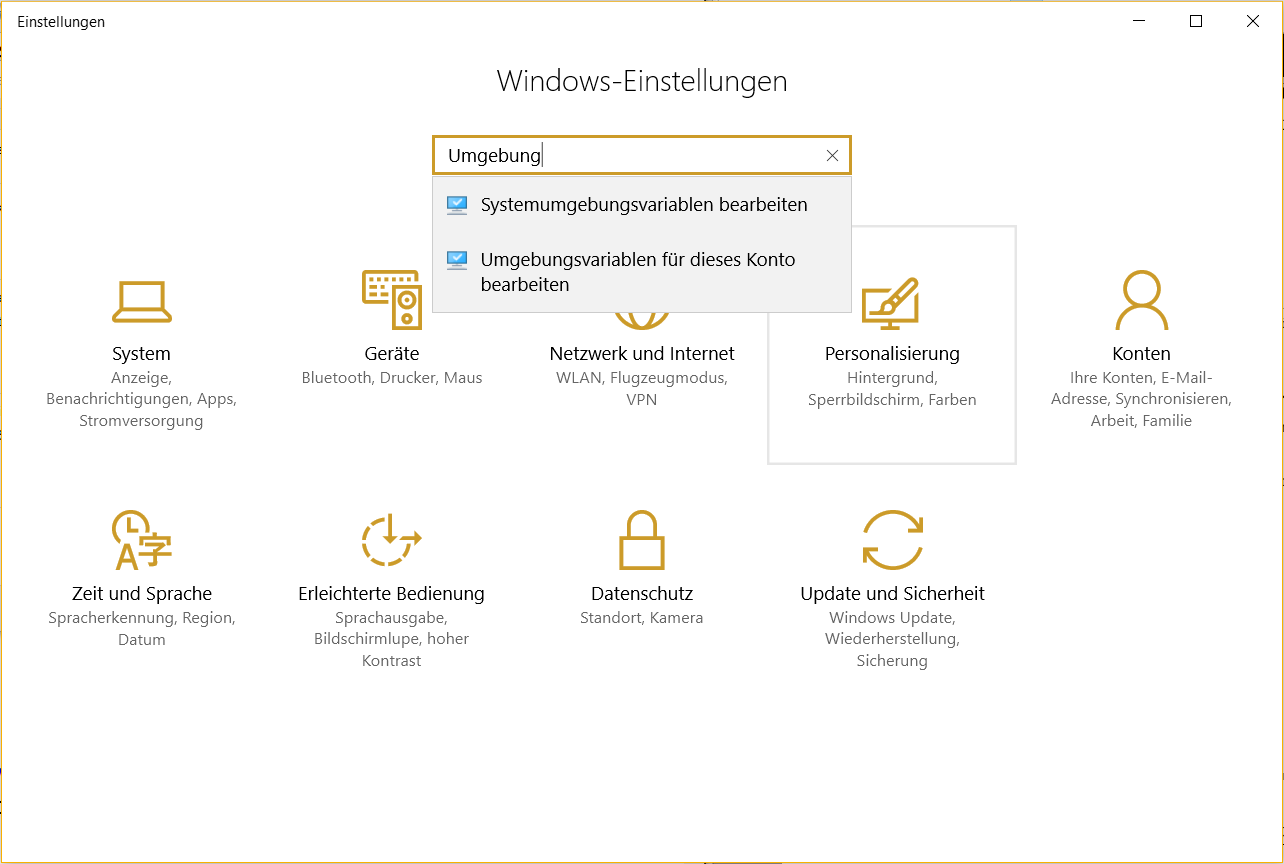
\includegraphics[width=0.8\textwidth]{Bilder/path-01}
\end{center}

\item Im sich öffnenden Dropdown-Menü wählt man entweder den Eintrag \enquote{Systemumgebungsvariablen bearbeiten} aus, wenn der Pfad für alle Nutzer des Rechners angepasst werden soll oder \enquote{Umgebungsvariablen für dieses Konto bearbeiten}, wenn der Pfad nur für den aktuellen Nutzer angepasst werden soll

\begin{center}
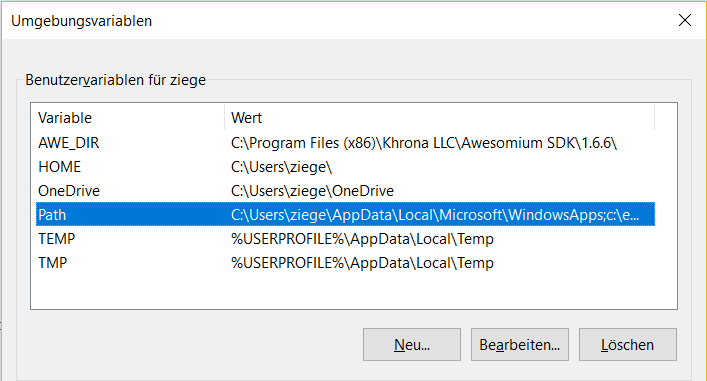
\includegraphics[width=0.8\textwidth]{Bilder/path-03}
\end{center}


\item Im \enquote{Umgebungsvariablen} Menü wählt man den Eintrag \enquote{Path} und geht auf \enquote{Bearbeiten}
\item Im folgenden Menü klickt man auf \enquote{Neu} und fügt den Pfad zur \texttt{Emacs.exe} -- bei mir \texttt{c:\textbackslash emacs\textbackslash bin} hinzu

\begin{center}
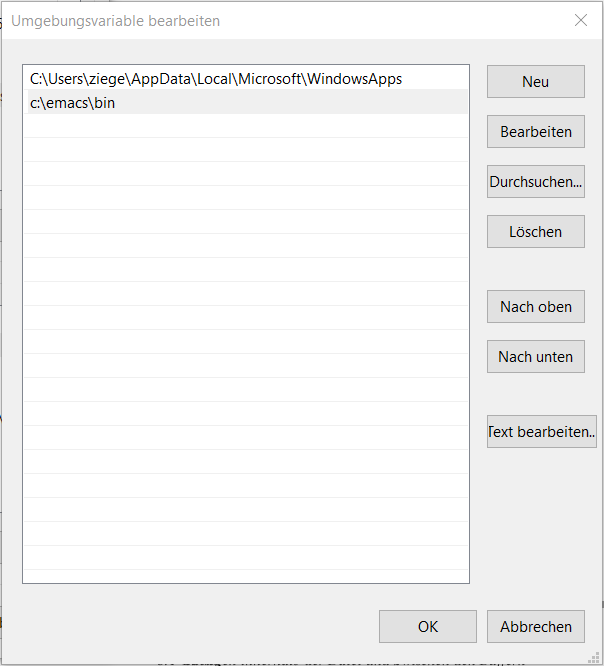
\includegraphics[width=0.8\textwidth]{Bilder/path-02}
\end{center}


\end{enumerate}

Startet man jetzt eine neue Eingabeaufforderung (aka \enquote{DOS-Box}), so kann man Emacs jetzt aus jedem Verzeichnis heraus starten, ein manueller Wechsel nach \texttt{c:\textbackslash emacs\textbackslash bin} ist nicht mehr notwendig.

\end{tcolorbox}

\begin{figure}
\begin{center}
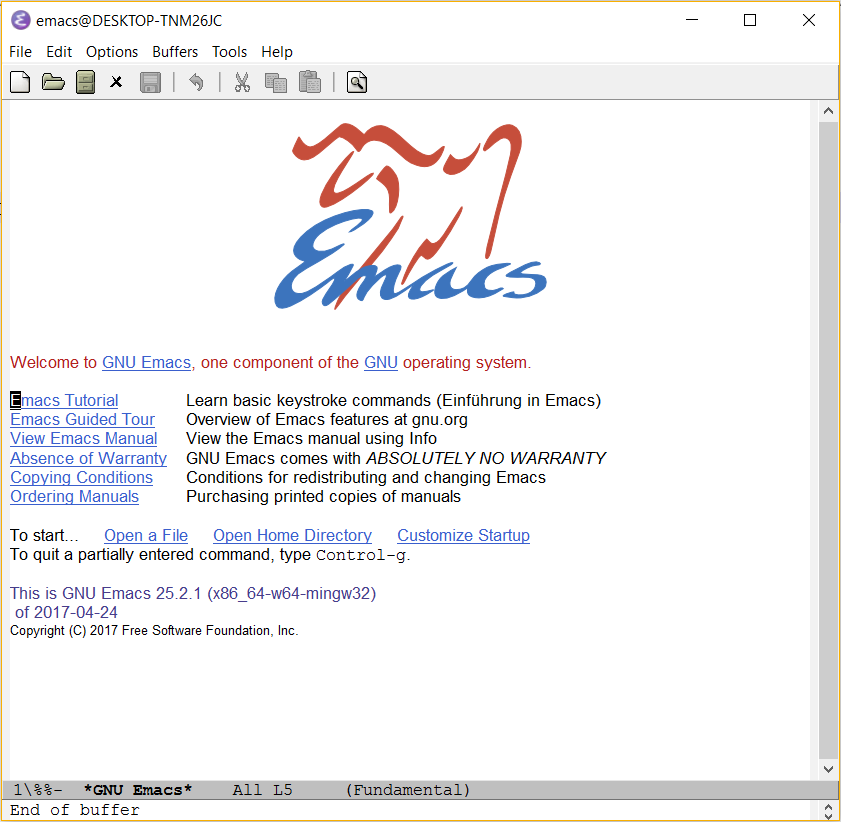
\includegraphics[width=\textwidth]{Bilder/emacs-01}
\caption{Emacs 25.2 nach dem Start}\label{fig:emacs-01}
\end{center}
\end{figure}

\begin{figure}
\begin{center}
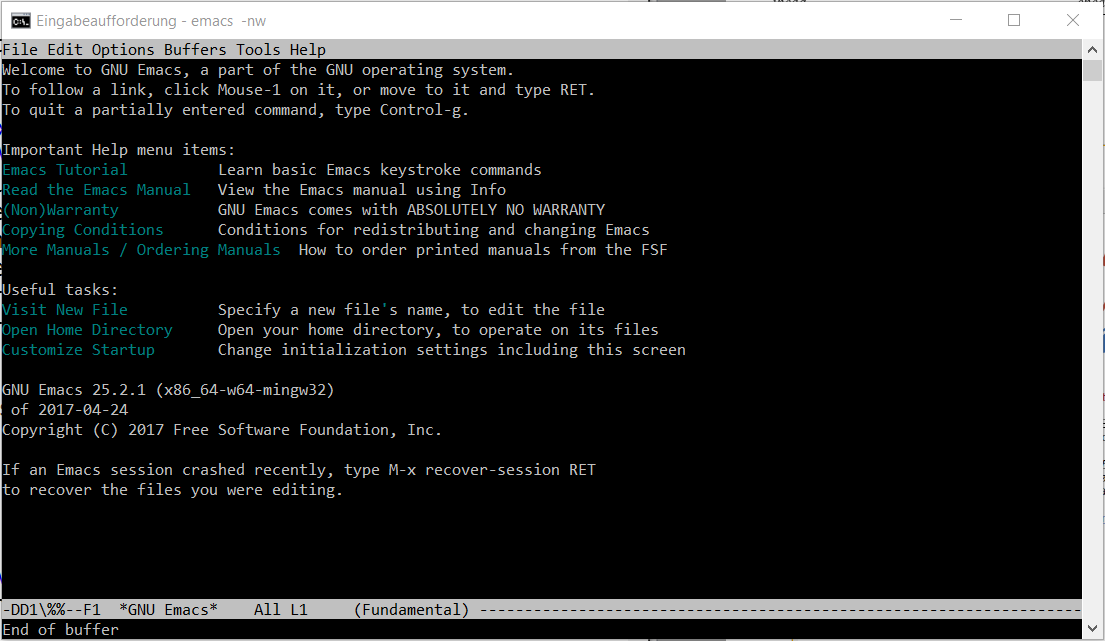
\includegraphics[width=\textwidth]{Bilder/emacs-02}
\caption{Emacs 25.2 nach dem Start im Kommandozeilenmodus}\label{fig:emacs-02}
\end{center}
\end{figure}


Beenden lässt sich Emacs ebenfalls auf verschiedene Arten:

\begin{itemize}
	\item Durch Drücken des Schließen-Knopfes
	\item Durch Ausführen des "Quit" Menü-Eintrags im \texttt{File}-Menü
	\item Durch Ausführen des Befehls  \LKeyAltX{x} \texttt{save-buffers-kill-terminal}
	\item Durch Ausführen der Tastensequenz \LKeyStrgX{x} \LKeyStrgX{c}; dies ist die vordefinierte Tastenkombination für \LKeyAltX{x} \texttt{save-buffers-kill-terminal}

\end{itemize}

In jedem dieser Fälle fragt Emacs nach, falls es noch Buffer gibt, die noch nicht gespeichert wurden. 
Wer in keinem Fall gefragt werden möchte, selbst wenn es noch ungesicherte Buffer gibt, kann \LKeyAltX{x} \texttt{kill-emacs} ausführen oder sogar -- was nicht empfehlenswert ist -- die Standardtastenkombination \LKeyStrgX{x} \LKeyStrgX{c} mit diesem Befehl überschreiben.

\section{Laden und Speichern}

Mittels Maus lädt man Dateien entweder über den Menüeintrag \enquote{Open File} im File-Menü oder durch Drücken des Öffnen-Symbols in der Symbolleiste, siehe folgendes Bild. Startet man Emacs von der Kommandozeile aus, so lässt sich der Dateiname auch als Parameter übergeben, wobei gilt: Ist die Datei nicht vorhanden, so wird ein entsprechender Buffer erzeugt, der beim Speichern eben diese Datei schreibt, wenn der User Schreibrechte hat.

Der eigentliche Emacs-Weg für das Öffnen liegt aber nicht darin, die Maus von A nach B zu schubsen, wie bei allen weiteren Aktionen gibt es auch hier entsprechende Tastenkombinationen. Im Fall des Öffnens bzw. Erstellens einer Datei lautet diese Tastenkombination \LKeyStrgX{x} \LKeyStrgX{f}, was ein Shortcut für den Befehl \texttt{find-file} ist, der auch über \LKeyAltX{x} \texttt{find-file} ausgeführt werden kann.

Zusätzlich zum Laden bzw. Erstellen eines Buffers über \texttt{find-file} gibt es noch die Möglichkeit, über \LKeyStrgX{x} \texttt{~b <Buffername>} einen Buffer neu zu erstellen, wenn noch kein Buffer dieses Namens im Speicher existiert.

Für das Speichern von Dateien bietet Emacs die folgenden Möglichkeiten an

\begin{itemize}
	\item die beiden Menü-Einträge im File-Menü, \enquote{Save} und \enquote{Save As}, um Dateien unter dem bisherigen Namen bzw. einem neuen Namen zu speichern
	\item das entsprechende Symbol in der Symbolleiste

\item \LKeyStrgX{x} \LKeyStrgX{s} für den Shortcut zum Befehl \texttt{save-buffer} 

\item \LKeyStrgX{x} \texttt{s} für den Shortcut zum Befehl \texttt{save-some-buffers}, was einem \enquote{Speichere alle Buffer} entspricht 
\item \LKeyStrgX{x} \LKeyStrgX{w} für den \enquote{Speichern als}-Befehl \texttt{write-buffer}
\item 
\item 
\item 
\end{itemize}


\section{Bewegen in der Datei und zwischen Buffern}

Befindet man sich in einem Buffer, kann man sich mit den Befehlen aus der folgenden Tabelle innerhalb des Buffers bewegen:

\begin{table}
\caption{Befehle zum Bewegen innerhalb des Buffers}\label{tab:moveinbuffer}
\begin{center}
\begin{tabular}{lll} \\ \toprule
Bewegung um & vor & zurück \\ \midrule
Zeichen & \LKeyStrgX{b} & \LKeyStrgX{f} \\ 
Wort & \LKeyAltX{b} & \LKeyAltX{f} \\
Zeile & \LKeyStrgX{p} & \LKeyStrgX{n} \\
Satz & \LKeyAltX{a} & \LKeyAltX{e} \\
Absatz & \LKeyAlt+\{ & \LKeyAlt+\}  \\
Seite & \LKeyStrgX{x} [ & \LKeyStrgX{x} ] \\ \bottomrule
\end{tabular}
\end{center}
\end{table}


 





\section{Editieren von Text}

\section{Suchen und Ersetzen}

\section{Das eingebaute Hilfesystem}



\section{Zusammenfassung}

Hier die wichtigsten Erkenntnisse des 


\chapter{Konfiguration}

% https://www.gnu.org/software/emacs/manual/html_node/efaq-w32/Location-of-init-file.html

\section{Manuelle Konfiguration von Paketen}

\section{Das Emacs-Paketsystem}

\section{use-package}

\chapter{Org Mode}

\chapter{Auc\TeX}

\chapter{Was sonst noch geht\ldots}

\section{ccrypt}

\section{GraphViz}

\section{Emacs als E-Mail-Programm}

\subsection{Emacs als RSS-Reader}

\section{Sweave}

\section{Spielen im Emacs}\label{sec:spielen}

\chapter{Programmierung}

\subsection{Das \enquote{Hello Emacs}-Beispiel}




\chapter{Weitere nützliche Software-Tools}

In diesem Kapitel sollen weitere nützliche Software-Tools vorgestellt werden, die im Zusammenhang mit Emacs interessant sind und von denen man zumindest gehört haben sollte. Denn \enquote{Hat man nur einen Hammer, so sieht alles wie ein Nagel aus!}	

Ergänzen oder ersetzen

\section{\TeX/\LaTeX}

\TeX\LaTeX\ ist ein professionelles Textsatzsystem, mit dem auch dieses Buch gesetzt wurde. Ähnlich alt wie Emacs nutzt \LaTeX\ Befehle, um den Text auszuzeichnen. Ein Compiler verwandelt dann den Text in PDF. Zur Installation empfiehlt es sich, die \TeX\ Live Distribution von \url{http://ww.tug.org} zu installieren. Ebenso wie den Pfad zur \texttt{emacs.exe} trägt man am besten auch den Pfad zu den \texttt{*latex.exe} Dateien in die PATH-Variable ein.

\subsection{Das erste \LaTeX-Dokument}

Das folgende Listing zeigt ein einfaches Beispiel für ein \LaTeX-Dokument. Gibt man den Text so mittels Emacs ein und übersetzt dann über Auc\TeX\ mit beispielsweise \texttt{pdflatex}, so sollte das PDF aus Abbildung \todo{Link} dabei entstehen. 


\subsection{Eine Musterpräsentation mit \texttt{Beamer}}

\LaTeX\ lässt sich auch vortrefflich für die Erstellung von Präsentationen nutzen. Das vermutlich fortschrittlichste Paket, \texttt{Beamer}, ist von Till Tantau. 

\subsection{Ein Musterbrief mit \texttt{scrlttr2}}


\subsection{Wer mehr wissen möchte\ldots}


Tabellensatz eigenes Buch, daher nur kurzer Überblick

Installiere TeX Live oder MikTeX, stelle sicher dass im Pfad vorhanden

Probiere das folgende Dokument aus und übersetze es auf der Kommandozeile.

Schnapp Dir ein Buch.

\section{sed und awk}

\section{VI(M)}



\backmatter

\blindtext

\begin{lstlisting}[basicstyle=\ttfamily] % <--- here
;; distraction-free
;;  https://nickhigham.wordpress.com/2016/01/14/distraction-free-editing-with-emacs/
(scroll-bar-mode 0)    ; Turn off scrollbars.
(tool-bar-mode 0)      ; Turn off toolbars.
(fringe-mode 0)        ; Turn off left and right fringe cols.
(menu-bar-mode 0)      ; Turn off menus.
;; bind fullscreen toggle to f9 key
(global-set-key (kbd "<f9>") 'toggle-frame-fullscreen)

;; http://emacs.stackexchange.com/questions/2999/how-to-maximize-my-emacs-frame-on-start-up
;; Start fullscreen (cross-platf)
(add-hook 'window-setup-hook 'toggle-frame-fullscreen t)
; emacs-doctor.com/emacs-strip-tease.html
;; Prevent the cursor from blinking
(blink-cursor-mode 0)
;; Don't use messages that you don't read
(setq initial-scratch-message "")
(setq inhibit-startup-message t)
\end{lstlisting}

\nocite{*}

\printbibliography 


\end{document}